\documentclass[twoside]{article}

\usepackage{amsmath}
\usepackage{amsfonts}
\usepackage{graphicx}
\usepackage{multirow}
\usepackage{fontspec}
\usepackage{hyperref}
\usepackage{xepersian}
% Font Settings ======================
\setlatintextfont{LinLibertine}[Path = fonts/latin/]
\settextfont{HMXKayhan}[
Path = fonts/fa/ ,
BoldFont = HMXKayhanBd]
% Graphic Settings ===================
\graphicspath{{images/}}
\DeclareGraphicsExtensions{.jpeg,.png,.jpg}


\title{\Huge گزارش آزمایش 6 آز مدار منطقی }
\author{\Large علی دهقانی ، ماهان بیهقی}
\date{دانشگاه صنعتی شریف}

\begin{document}
	\maketitle
	\newpage
	\section*{نام آزمایش}
	تایمر ماشین لباسشویی
	
	\section*{اهداف آزمایش}
	پیاده سازی یک یک تایمر برای ماشین لباسشویی
	
	\section*{شرح آزمایش}
	
	\subsection*{لیست تراشه ها و قطعات مورد نیاز} 
	\begin{itemize}
		\item
		\href{https://www.ti.com/lit/ds/symlink/sn74f163a.pdf?ts=1672133706533&ref_url=https%253A%252F%252Fwww.google.com%252F}{74163 FOUR BIT BINARY COUNTER}
		\item
		\href{https://datasheetspdf.com/pdf/248156/NationalSemiconductor/74154/1}{74154 DECODER/DEMULTIPLEXER}
		\item
		\href{https://cdn.datasheetspdf.com/pdf-down/7/4/0/7400_FairchildSemiconductor.pdf}{7400 QUAD TWO-INPUT NANAD}
	\end{itemize}
	
	\subsection*{شرح آزمایش}
	این ماشین لباسشویی دو برنامه شستشو با آب گرم و آب سرد دارد که با تغییر وضعیت کلید مشخص میشود. 
	
	در برنامه شستشو با آب سرد به ترتیب مراحل آبگیری ، شستشو ، تخلیه و سپس خشک کردن در مدت زمان 2 و 3 و 2 و 2 پالس ساعت انجام میشود.
	
	در برنامه شستشو با آب گرم به ترتیب مراحل آبگیری ، گرم کردن آب ، شستشو ، تخلیه و خشک کردن در مدت زمان 2 و 3 و 3 و 2 و 2 پالس ساعت انجام میشود.
	
	با زدن کلید کار ماشین لباس شویی شروع میشود ، به شرط آنکه شیر آب باز و در ماشین لباس شویی بسته باشد و برنامه مورد نظر انتخاب شده باشد.
	
	سیگنال های ورودی مدار : کلید شروع ، باز و بسته بودن شیر آب ، باز و بسته بودن در ماشین ، انتخاب عملیات آب سرد یا گرم
	
	سیگنال های خروجی مدار : شستشو ، گرم کردن آب ، عملیات آبگیری ، تخلیه و خشک کردن
	
	
	
	\subsection*{مراحل آزمایش و مدارات}
	از تراشه 74163 به عنوان یک شمارنده 4 بیتی استفاده کرده ایم. این تراشه جایگزین تراشه 74192 در مدار پیش گزارش شده است تا کمبود شمارش 10 تا 15 را برطرف کند.
	
	همچنین از تراشه 74154 که یک دیکودر 4 به 16 است برای تبدیل خروجی شمارنده چهار بیتی به عملیات موردنظر استفاده شده است. این تراشه نیز جایگزین تراشه 74138 پیش گزارش شده است تا پیچیدگی مدار کاهش یابد.(برای پیاده سازی مدار با تراشه 74138 به 4 تراشه نیاز است ولی با تراشه 74154 تعداد تراشه های موردنیاز 2 خواهد بود) 
	
	برای شروع به کار مدار باید هر سه کلید مربوط به روشن و خاموش بودن ، باز بودن شیر آب و بسته بودن درب ماشین در حالت 1 باشند. همچنین با قرار دادن کلید آب گرم شستشو با آب گرم انجام میشود و در غیر اینصورت برنامه شستشو با آب سرد اجرایی میشود. 
	در هر مرحله از اجرا اگر یکی از کلید های باز و بسته بودن درب یا باز بودن شیر آب قطع شوند ، اجرا متوقف میشود و در صورت برگرداندن به حالت اولیه ، اجرا برنامه ادامه میابد.

	برای نشان دادن مرحله فعلی شستشو از 5 دیود نوری استفاده شده است که در بازه های زمانی تعریف شده روشن خواهند بود.
	فایل ارسالی همراه با این داکیومنت فایل پروژه موردنظر است و شکل زیر شمای کلی مدار را نشان میدهد.

	\begin{figure}[h!]
		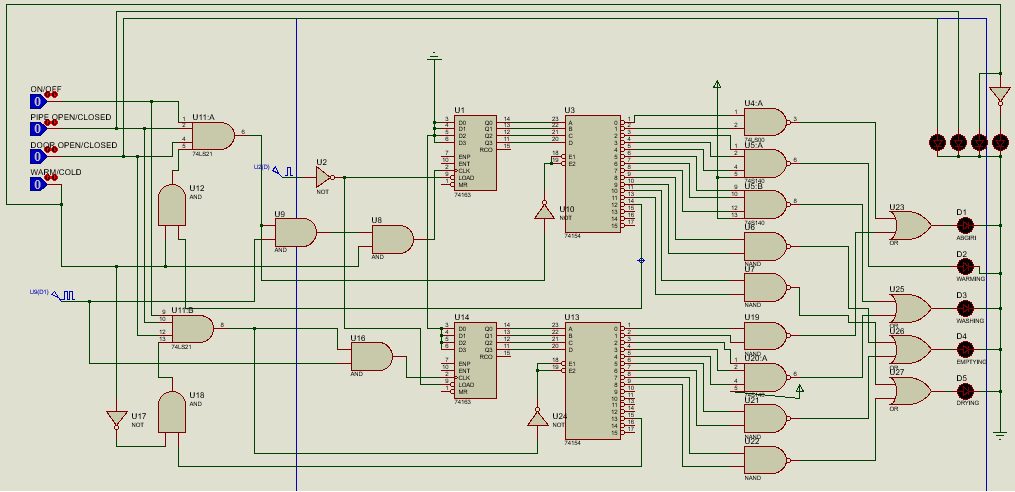
\includegraphics[scale=0.50]{images/madar.png}
		\caption{طرح پیشنهادی برای مدار}

	\end{figure}
\end{document}







